\section{CNN}
\noindent 1、卷积层(Convolutional Layers):

使用了五个卷积层,每一层包括卷积操作(nn.Conv2d)、批量归一化(nn.Batch\\Norm2d)、激活函数(ReLU)和最大池化(nn.MaxPool2d)。
卷积核大小为 (3, 3),步长(stride)为 1,padding 模式为 'same',保证了卷积后特征图大小不变。

\noindent 2、Dropout 层:

在第二、四、五个卷积层后使用了 Dropout 操作,有助于防止过拟合。

\noindent 3、全连接层(Fully Connected Layers):

包括两个全连接层,每一层包括全连接操作(nn.Dense)、激活函数(ReLU)和 Dropout 操作。
第一个全连接层的输出大小为 128,输入大小为 6400(由 nn.Flatten 层展平得到)。
第二个全连接层的输出大小为 3,对应于分类的类别数量。

\noindent 4、激活函数:

使用了 ReLU 激活函数,除了最后一层,最后一层使用了 Softmax 激活函数进行多类别分类。
打印操作:

在网络中使用了 P.Print() 操作,该操作用于在计算过程中打印张量的形状信息。
网络的整体结构是卷积层的堆叠,通过不断降低特征图的大小,最终通过全连接层输出分类结果。 Dropout 层有助于提高模型的泛化能力。
\begin{figure}[H]
	\centering
	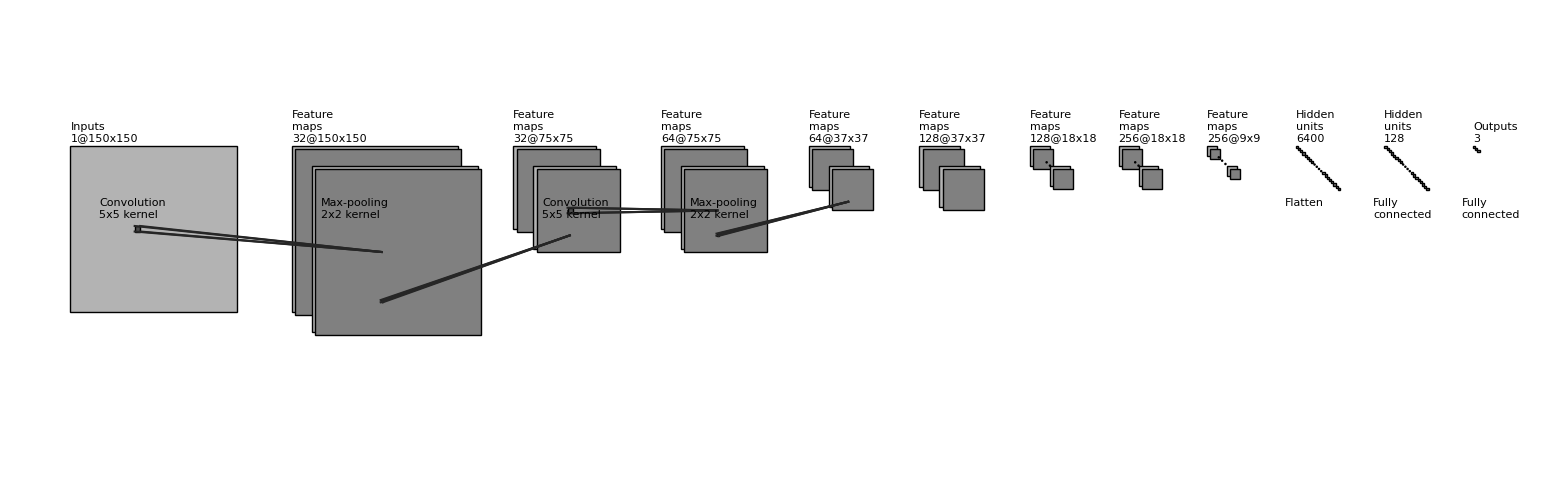
\includegraphics[width=1\textwidth]{convnet_fig.png}
	\caption{CNN网络图像}
	\label{fig:example}
\end{figure}
